\chapter{Theory}


We are doing some friction eztimates

\section{Vehicle Dynamics}

Bla bla \cite{fordonsdynamik}

Bla bla \cite{pacejka}

\section{Tire Dynamics}

A tire that is non loaded will have a radius called unloaded radius. When a tire is loaded, and therefore have a normal force acting from the ground, it will deform against the contact area to the ground. This deformation will lead to a shorter radius to the ground, called the effective rolling radius. 

\subsection{Longitudinal forces}

Without torque acting on the tire, there will be rolling resistance due to higher compressing in the tire/road compression area then in the expansion area.
\begin{equation}
 	RollingResistance = \frac{F_{resistance}}{F_{z}}
\end{equation}
When a longitudinal force is acting on the tire, traction or braking, the tire will have more compression/expansion and a slip will occur. The longitudinal slip is defined as
\begin{equation}
	 \kappa = \dfrac{R_{e}\omega-V_{x}}{V_{x}}
\end{equation}
Where $V_{x}$ is the nominal velocity, $R_{e}$ the effective rolling radius, and $\omega$ the angular velocity of the wheel.

The longitudinal force that will be acquired depends on the normal force, $ F_{N} $ and the friction used, $ \mu(s) $.
\begin{equation}
	 F_{x} = F_{z}\mu(s)
\end{equation}
The used friction will increase with the slip ratio until the maximum friction is met. This is when full gliding occurs. 

\subsection{Lateral forces}

Cornering stiffness
\begin{equation}
	C_{y} = \frac{\delta F_{y}}{\delta}
\end{equation}
Where $\delta$ is the steering wheel angle.

Self aligning torque
\begin{equation}
	M_{z} = F_{y}t_{p}
\end{equation}
Where $ F_{y} $  is the lateral force acting on the tire and $ t_{p} $ its distance to the center of the wheel. 

The lateral force acting on the wheel depends on its slip angle
\begin{equation}
	F_{y}=C_{F}\alpha
\end{equation}

\section{Tire Models}

There are several models to describe a tire mathematically. These models can be divided into four categories, empirical models, similarity models, simple physical models and complex physical  models. In Figure \ref{tire_modeling} some modeling characteristics and how they behave depending on category can be seen.

\begin{figure}[h]
	\centering
	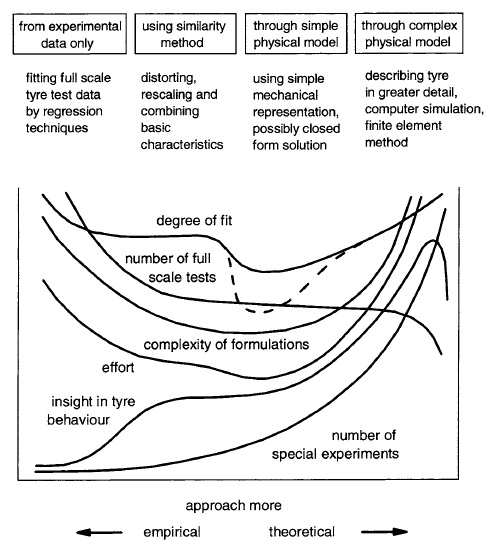
\includegraphics[width=0.8\textwidth]{Pictures/tire_modeling}
	\caption{Four categories of possible types of approach to develop a tire model. \cite{pacejka}}
	\label{tire_modeling}
\end{figure}


\subsection{Brush Model}



\section{Differentials}

\subsection{Open differential}

\subsection{Limited slip differential}

\subsection{FXD}